\documentclass[11pt]{article}
\usepackage[utf8]{inputenc}

\usepackage{amsmath}
\usepackage{amssymb}
\usepackage{setspace}
\usepackage{graphicx}
\usepackage{float}

\newcommand{\blank}{\enspace}
\newcommand{\blankt}{\text{ }}
\newcommand{\sttensor}{\text{ }{\scriptscriptstyle ^{^{(\mathcal{M})}}}}

\doublespacing

\title{GHGFort; A Fortran Library For The Generalized Harmonic Gauge Formulation of General Relativity}
\author{Alexander Buchanan}
\date{}
\numberwithin{equation}{section}
\begin{document}

\maketitle

\begin{abstract}
    I present two derivations of the two most common approaches of numerical relativity, the $3+1$ formulation utilized by the ADM and BSSN approach following that done by Baumgarte and Shapiro \cite{baumgarte_shapiro_2010}, and the general harmonic gauge approach. Where both of these derivations are necessary for understanding numerical relativity and deriving proper equations that can be integrated. These derivations are then used to write a numerical library, GHGFort, that solves the Einstein field equations in the general harmonic gauge. I present a discussion of how to put the equations in the computer, as well as a test case of propagating a gravitational wave through space--time as a proof of concept of the code.  
\end{abstract}

\tableofcontents

\section{Introduction}
In 1916, Albert Einstein presented his theory of General Relativity, a new theory of gravity. Einstein proposed that gravity was not a force, as the Newtonian theory suggested, but was rather a manifestation of geometrical properties of the universe induced by mass. Using the equivalence principle, which states the equivalence of inertial and gravitational mass \cite{schutz}, Einstein was able to derive the Einstein Field Equations:
\begin{equation}\label{EFEintro}
G_{\mu\nu} = 8\pi T_{\mu\nu}.
\end{equation}
This equation is defined on a space--time manifold $\mathcal{M}$, which is semi--Riemannian, and has metric tensor $g_{\mu\nu}$. 

In equation (\ref{EFEintro}), which uses normal units of $c=G=1$, $G_{\mu\nu}$ is defined as the Einstein tensor,
and $T_{\mu\nu}$ is the stress energy tensor.
Here the Einstein tensor is a tensor that is purely geometric, defined as
\begin{equation}
    G_{\mu\nu} = R_{\mu\nu} - \frac12g_{\mu\nu}R
\end{equation}
where $R_{\mu\nu}$ is the Ricci tensor, a contraction of the Riemann tensor, and $R$ is the the Ricci scalar, a contraction of the Ricci tensor. 

These equations equate curvature of space--time and energy and mass present in the space--time, that is, in the words of John Wheeler, ``Mass tells space-time how to curve, and space-time tells mass how to move." With this relationship, it is possible to calculate the high energy limit of gravitational events where Newton's theory fails. 

These equations are nonlinear and in general very difficult to solve analytically. There are however solutions to the field equations, such as the Minkowski space--time, which reduces the theory back down its special relativistic case. A less trivial solution was discovered a year after Einstein published his initial findings. Karl Schwarzschild derived a solution that describes a spherically symmetric static mass in space--time. The Schwarzschild solution also implied the existence of a massive object, where space--time curved so drastically that within a certain radius, termed the event horizon, photons would not be able to escape the gravitational pull. That object is now referred to as a black hole, which has recently been the interest of the gravitational experiments LIGO \cite{LIGOPAPER1} and VIRGO \cite{2017ApJ...851L..35A}.  

Einstein's equations also can predict the expansion of the universe by adding a single term, the cosmological constant $\Lambda$ multiplied by the metric, to equation (\ref{EFEintro}),
\begin{equation}\label{EFEcosmo}
    G_{\mu\nu} + \Lambda g_{\mu\nu} = 8\pi T_{\mu\nu}.
\end{equation}
This cosmological expansion can be quantified by the Friedmann–-Lemaître–-Robertson–-Walker metric, where this solution to the Einstein equations agrees with Edwin Hubble's finding that the universe is isotropically expanding.

While many solutions to the Einstein field equation exist, more complex systems becomes highly nonlinear, and impossible to solve analytically. Such as in the instance of binary inspiral mergers of massive bodies near the merger point. To analyze these problems, numerical simulations of the Einstein field equations are required, and in recent years approaches to these problems have been presented and successfully used to simulate these astrophysical events.


\section{Numerical Relativity}
Numerical relativity is a relatively new field that aims to take on the subject of simulating highly complex nonlinear astrophysical events such as binary black hole mergers. The general approach to the issue is to write Einstein's equations in such a way that the time derivatives of the equations can be successfully separated from the spatial derivatives, allowing for direct numerical integration of the equations. 

Currently, there are two main methods of approach. The first and most popular is the $3+1$ approach, which takes the approach of decomposing, or foliating the space--time manifold $\mathcal{M}$ into a spatial portion and a time portion. The second is the general harmonic gauge approach, where the coordinates on $\mathcal{M}$ must satisfy the general harmonic gauge, allowing the Einstein field equations to be written as a nonlinear wave equation, which can then be directly integrated. 

The most popular approach is a $3+1$ approach using the BSSN formalism. This formalism allows for stable numerical simulation of the Einstein equation over long periods of time. While the BSSN equations might be the most popular, the general harmonic gauge approach is equally valid and has been successfully used to simulate the Einstein field equations \cite{2005CQGra..22..425P}. These formalism's have wide implications in the field of relativity, such as being used in combination with relativistic hydrodynamic codes that can be used to analyze and understand the neutron binary star merger recently detected by LIGO \cite{2041-8205-848-2-L13}.

The following section presents the basic derivation of the $3+1$ formulation and the general harmonic gauge. The $3+1$ formulation is derived first as it has constructs which the generalized harmonic gauge utilizes in its derivation. 

\subsection{The 3+1 Formulation}

Following the derivation in \cite{baumgarte_shapiro_2010}, the formulation arises by foliating space--time into spacelike hypersurfaces $\Sigma$, which are level surfaces of a global time function, $t$. Given a scalar time function $t$, a covector field denoted 
\begin{equation}\label{covectorfield}
    \Omega_{\mu} = \nabla_{\mu}t
\end{equation}
may be defined where $\nabla_{\mu}$ is a covariant derivative. 
Then defining an arbitrary space--time metric $g_{\mu\nu}$, the norm of the covector field may be written as
\begin{equation}
    \rvert\rvert \Omega \rvert\rvert^2 = g^{\mu\nu}\nabla_{\mu}t\nabla_{\nu}t.
\end{equation}
This norm of the covector field defines what is called the lapse function, $\alpha$. The lapse is a function that measures proper time elapsed between subsequent hypersurfaces $\Sigma$ where 
\begin{equation}
    \rvert\rvert \Omega \rvert\rvert^2 = \frac{-1}{\alpha^2}
\end{equation}
Therefore the normalized covector field is given by
\begin{equation}\label{normalizedcovectorfield}
    \omega_{\mu} = \alpha\Omega_{\mu} 
\end{equation}
and the unit normal to the hypersurface $\Sigma$
\begin{equation}
    n^{\mu} = g^{\mu\nu}\omega_{\nu}
\end{equation}
where $n^{\mu}$ points in the direction of increasing time, and is normalized and time-like 
\begin{align}
    n^{\alpha}\omega_{\beta} &= -g^{\mu\nu}\omega_{\nu}\omega_{\mu} = -\omega^{\mu}\omega_{\mu} = 1 \\
    n^{\mu}n_{\mu} &= g^{\mu\nu}\omega_{\nu}g_{\mu\nu} \omega^{\nu} = \omega^{\mu} \omega_{\mu} = -1. \label{normalcontract}
\end{align}

An induced metric is defined using these normal vectors such that it is a projection perpendicular $n^{\mu}$,
\begin{equation}
    \gamma^{\mu\nu} = g^{\mu\nu} + n^{\mu}n^{\nu}
\end{equation}
With these constructions, it is now possible to break space--time tensors into their purely spatial part on $\Sigma$ and their time-like part. Defining two projection operators \cite{baumgarte_shapiro_2010} ,
\begin{align}
    \gamma^{\mu}_{\blank\nu} &= g^{\mu}_{\blank\nu} + n^{\mu}n_{\nu} \\
    -n^{\mu}n_{\nu} &= \delta^{\mu}_{\blank\nu} + \gamma^{\mu}_{\blank\nu}.
\end{align}
With these projection operators any arbitrary 4-dimensional tensor can be projected onto $\Sigma$ by contracting each index with the projection operator. 

The projection operators are also used to define a 3-dimensional covariant derivative that takes 3-dimensional tensors to 3-dimensional tensors. It is defined by projecting the index of the covariant derivative, as well as each index of the tensor onto $\Sigma$. For a scalar function f, this is given trivially as
\begin{equation}
    D_{\mu}f = \gamma_{\mu}^{\blank\nu} \nabla_{\nu}f
\end{equation}
and for a rank (1,0) and rank (2,0) tensor is is given by
\begin{align*}
    D_{\mu}v_{\alpha} &= \gamma_{\mu}^{\blank\tau} \gamma_{\alpha}^{\blank\sigma} \nabla_{\tau} v_{\sigma} \\
    D_{\mu}T_{\alpha\beta} &= \gamma_{\mu}^{\blank\nu} \gamma_{\alpha}^{\blank\sigma} \gamma_{\beta}^{\blank\tau} \nabla_{\nu} T_{\sigma\tau}
\end{align*}
where other tensors of differing rank follow similarly.

This 3-dimensional covariant derivative can be expressed in terms of 3-dimensional Christoffel symbols defined using the induced metric, $\gamma_{\mu\nu}$,
\begin{equation}
    \Gamma^{\alpha}_{\blank\mu\nu} = \frac12 \gamma^{\alpha\tau}\left(\gamma_{\tau\mu,\nu} + \gamma_{\tau\nu,\mu} - \gamma_{\mu\nu,\tau}\right).
\end{equation}
This Christoffel symbol then can be used to define a 3-dimensional Riemann tensor, Ricci tensor, and Ricci scalar. 

These tensors alone, while describing $\Sigma$, do not satisfy the requirements of the Einstein field equations which requires a 4-dimensional stress-energy tensor. Therefore these 3-dimensional tensors only provide information about the intrinsic curvature of $\Sigma$ at some time, but lack information about the geometry of the space--time manifold $\mathcal{M}$ required by the theory. Therefore the extrinsic curvature must be derived.  

The extrinsic curvature is given by the tensor \cite{baumgarte_shapiro_2010}, \cite{poisson}
\begin{equation}
    K_{\mu\nu} \equiv  - \gamma_{\blank\mu}^{\tau} \gamma_{\blank\nu}^{\sigma} \nabla_{\sigma}n_{\tau}
\end{equation}
and is by definition symmetric and spatial.

Given the extrinsic curvature the relationship between the 4-dimensional Riemann tensor, and the 3-dimensional Riemann tensor can be shown. This relationship follows from the Gauss--Codazzi equations. space--time tensors are super-scripted with an $(\mathcal{M})$ before them, whereas spatial tensors appear as normal. 
\begin{align}
     \gamma_{\mu}^{\blank\alpha} \gamma_{\nu}^{\blank\beta} \gamma_{\sigma}^{\blank\gamma} \gamma_{\tau}^{\blank\delta}\blank \sttensor R_{\alpha\beta\gamma\delta} &= R_{\mu\nu\sigma\tau} + K_{\mu\sigma}K_{\nu\tau} - K_{\mu\tau}K_{\sigma\nu} \label{Gausseq}\\
    \gamma_{\mu}^{\blank\alpha} \gamma_{\nu}^{\blank\beta} \gamma_{\sigma}^{\blank\gamma} n^{\blank\delta}\blank \sttensor R_{\alpha\beta\gamma\delta} &= D_{\nu}K_{\mu\sigma} - D_{\mu} K_{\nu\sigma}. \label{Codazzieq}
\end{align}


There is then a need for a an equation that resembles a time derivative of the extrinsic curvature, the Ricci equation gives this notion by taking the Lie derivative of the extrinsic curvature in the $n^{\mu}$ direction, 
\begin{equation} \label{RicciEq}
    \mathcal{L}_{\textbf{n}}K_{\mu\nu} = n^{\alpha} n^{\gamma} \gamma_{\mu}^{\blank\delta} \gamma_{\nu}^{\blank\beta} \text{ } {\scriptscriptstyle ^{^{(\mathcal{M})}}}R_{\alpha\beta\gamma\delta} - \frac{1}{\alpha} D_{\mu} D_{\nu} \alpha - K^{\blank\gamma}_{\mu} K_{\nu\gamma}.
\end{equation}
This Lie derivative gives a derivative that appears to be a ``time'' derivative, allowing for the evolution equations to be written. 

Recalling the Einstein field equations, 
\begin{equation} \label{newEFE}
    G_{\mu\nu} \equiv \sttensor R_{\mu\nu} - \frac12\sttensor R g_{\mu\nu} = 8\pi T_{\mu\nu},
\end{equation}
the Gauss--Codazzi equations (\ref{Gausseq},\ref{Codazzieq}) and the Ricci equation (\ref{RicciEq}) can be used to replace the 4-dimensional Riemann tensor with its 3-dimensional counterpart allowing these geometric constructs to relate to the matter and energy portions of space--time. 

It remains to find a constraint equation for these evolution equations. Contracting the Gauss equation (\ref{Gausseq}) yields,
\begin{align}
    \gamma^{\mu\sigma} \gamma_{\mu}^{\blank\alpha} \gamma_{\nu}^{\blank\beta} \gamma_{\sigma}^{\blank\gamma} \gamma_{\tau}^{\blank\delta} \sttensor R_{\alpha\beta\gamma\delta} &= \gamma^{\mu\sigma} R_{\mu\nu\sigma\tau} + \gamma^{\mu\sigma} K_{\mu\sigma} K_{\nu\tau} - \gamma^{\mu\sigma} K_{\mu\tau} K_{\gamma\nu} \\
    \gamma^{\alpha\beta} \gamma_{\nu}^{\blank\gamma} \gamma_{\tau}^{\blank\delta} \sttensor R_{\alpha\beta\gamma\delta} &= R_{\nu\tau} + K K_{\nu\tau} - K^{\sigma}_{\blank\tau} K_{\sigma\nu} \label{contractgauss}
\end{align}
where $K$ is the trace of the extrinsic curvature. Then contracting once more,
\begin{align}
    \gamma^{\nu\tau} \gamma^{\alpha\beta} \gamma_{\nu}^{\blank\gamma} \gamma_{\tau}^{\blank\delta} \sttensor R_{\alpha\beta\gamma\delta} &= \gamma^{\nu\tau} R_{\nu\tau} + \gamma^{\nu\tau} K K_{\nu\tau} - \gamma^{\nu\tau} K^{\sigma}_{\tau}K_{\sigma\nu} \\
    \gamma^{\alpha\beta} \gamma^{\gamma\delta} \sttensor R_{\alpha\beta\gamma\delta} &= R + K^2 - K^{\sigma\nu}K_{\sigma\nu} \label{contract2gauss}
\end{align}
yields an expression for the space--time Riemann tensor in terms of the Ricci scalar on $\Sigma$ and the extrinsic curvature. The left hand side of \ref{contract2gauss} can be expanded,
\begin{align}
    &(g^{\alpha\beta} + n^{\alpha}n^{\beta})(g^{\gamma\delta} + n^{\gamma}n^{\delta})\sttensor R_{\alpha\beta\gamma\delta}  \\ &= (g^{\alpha\beta}g^{\gamma\delta} + 2g^{\beta\delta}n^{\alpha}n^{\gamma} + n^{\alpha}n^{\beta}n^{\gamma}n^{\delta}) \sttensor R_{\alpha\beta\gamma\delta} \\ &= \sttensor R + 2n^{\alpha}n^{\gamma} \sttensor R_{\alpha\gamma} \label{28}
\end{align}
Where the symmetries of the Riemann tensor imply $n^{\alpha}n^{\beta}n^{\gamma}n^{\delta} \sttensor R_{\alpha\beta\gamma\delta} = 0$. 

Now observing that the Einstein tensor can be written as
\begin{align}
\begin{split}
    G_{\mu\nu} &= R_{\mu\nu} - \frac12R(\gamma_{\mu\nu} - n_{\mu}n_{\nu}) \\
               &= R_{\mu\nu} - \frac12 R\gamma_{\mu\nu} + \frac12R n_{\mu}n_{\nu} 
               \end{split}
\end{align}
then according to (\ref{normalcontract}), multiplying both sides by $n^{\mu} n^{\nu}$,
\begin{align}
\begin{split}
    n^{\mu}n^{\nu}G_{\mu\nu} &= n^{\mu}n^{\nu}R_{\mu\nu} - \frac12 Rn^{\mu}n^{\nu}\gamma_{\mu\nu} + \frac12R n^{\mu}n^{\nu}n_{\mu}n_{\nu} \\ &= n^{\mu}n^{\nu}R_{\mu\nu} - \frac12 Rn^{\mu}n^{\nu}\gamma_{\mu\nu} + \frac12R n^{\mu}n^{\nu}n_{\mu}n_{\nu} \\ &= n^{\mu}n^{\nu}R_{\mu\nu} + \frac12R
\end{split}
\end{align}
which is a factor of 2 difference from (\ref{28}). Therefore since
\begin{equation}
    2n^{\mu}n^{\nu}G_{\mu\nu} = \gamma^{\alpha\beta} \gamma^{\gamma\delta} \sttensor R_{\alpha\beta\gamma\delta} 
\end{equation}
and using (\ref{contract2gauss}),
\begin{equation}
    2n^{\mu}n^{\nu}G_{\mu\nu}= R + K^2 - K^{\mu\nu}K_{\mu\nu}.
\end{equation}
Multiplying the right hand side of the Einstein field equations by the same factor of $2n^{\mu}n^{\nu}$, 
\begin{equation}\label{efeRHS}
    2n^{\mu}n^{\nu}G_{\mu\nu} = 2n^{\mu}n^{\nu}8\pi T_{\mu\nu} = 16\pi n^{\mu}n^{\nu}T_{\mu\nu}
\end{equation}
which can be written as,
\begin{equation}\label{hamiltonianconstraint}
    R + K^2 - K^{\mu\nu}K_{\mu\nu} = 16\pi n^{\mu}n^{\nu}T_{\mu\nu}.
\end{equation}
Equation (\ref{hamiltonianconstraint}) is the Hamiltonian constraint equation. 

One more constraint equation is required. A contraction of the Codazzi equation (\ref{Codazzieq}) yields, 
\begin{align}
\begin{split}
    \gamma^{\nu\sigma}D_{\nu}K_{\mu\sigma} - \gamma^{\nu\sigma}D_{\mu}K_{\nu\sigma} &= \gamma^{\nu\sigma} \gamma_{\mu}^{\blank\alpha} \gamma_{\nu}^{\blank\beta} \gamma_{\sigma}^{\blank\gamma} n^{\delta} \sttensor R_{\alpha\beta\gamma\delta} \\ 
    D_{\nu}K_{\mu}^{\blank\nu} - D_{\mu}K&= \gamma_{\mu}^{\blank\alpha} \gamma^{\beta\gamma} n^{\delta} \sttensor R_{\alpha\beta\gamma\delta} \label{contractedcodazzi}
\end{split}
\end{align}
where the right hand side can be expanded.
\begin{align} \label{expandedRHScodazzi}
    \begin{split}
    \gamma_{\mu}^{\blank\alpha} \gamma^{\beta\gamma} n^{\delta} \sttensor R_{\alpha\beta\gamma\delta} &= -\gamma_{\mu}^{\blank\alpha}(g^{\beta\gamma} + n^{\beta}n^{\gamma}) n^{\delta}\sttensor R_{\alpha\beta\gamma\delta} \\ 
    &= -\gamma_{\mu}^{\blank\alpha} n^{\delta} \sttensor R_{\alpha\delta} - \gamma_{\mu}^{\blank\alpha}n^{\beta}n^{\gamma}n^{\delta} \sttensor R_{\alpha\beta\gamma\delta} \\
    &= -\gamma_{\mu}^{\blank\alpha}n^{\delta} \sttensor R_{\alpha\delta}
    \end{split}
\end{align}
where $\gamma_{\mu}^{\blank\alpha}n^{\beta}n^{\gamma}n^{\delta} \sttensor R_{\alpha\beta\gamma\delta} = 0$ because of symmetries in the Riemann tensor. \cite{baumgarte_shapiro_2010}. Contracting the Einstein tensor with $\gamma_{\mu}^{\blank\alpha}n^{\delta}$ gives
\begin{align}
    \begin{split}
    \gamma_{\alpha}^{\blank\mu}n^{\nu} G_{\mu\nu} &= \gamma_{\alpha}^{\blank\mu}n^{\nu} \sttensor R_{\mu\nu} - \gamma_{\alpha}^{\blank\mu}n^{\nu} \frac12 \sttensor R g_{\mu\nu} \\ &= \gamma_{\alpha}^{\blank\mu}n^{\nu} \sttensor R_{\mu\nu} - \frac12 \sttensor R \gamma_{\alpha\nu}n^{\nu} \\ 
    &= \gamma_{\alpha}^{\blank\mu}n^{\nu} \sttensor R_{\mu\nu}
    \end{split}
\end{align}
where $\gamma_{\alpha\nu}n^{\nu} = 0$ by definition. Therefore equation (\ref{expandedRHScodazzi}) can be written as 
\begin{equation}
\gamma_{\mu}^{\blank\alpha} \gamma^{\beta\gamma} n^{\delta} \sttensor R_{\alpha\beta\gamma\delta} = -\gamma_{\mu}^{\blank\sigma}n^{\nu} G_{\sigma\nu}
\end{equation}
where then equation (\ref{contractedcodazzi}) becomes
\begin{equation}
    D_{\nu}K_{\alpha}^{\blank\nu} - D_{\alpha}K = -\gamma_{\alpha}^{\blank\mu}n^{\nu} G_{\mu\nu}.
\end{equation}
Once again, multiplying both sides of equation (\ref{newEFE}) by $-\gamma_{\alpha}^{\blank\mu}n^{\nu}$ the equation becomes
\begin{equation}\label{momentumconstraint}
    D_{\nu}K_{\alpha}^{\blank\nu} - D_{\alpha}K = -8\pi\gamma_{\alpha}^{\blank\mu}n^{\nu}T_{\mu\nu}.
\end{equation}
This is called the momentum constraint equation. 

The Hamiltonian constraint (\ref{hamiltonianconstraint}) and momentum constraint (\ref{momentumconstraint}) are both equations involving purely the induced metric $\gamma_{\mu\nu}$, and the extrinsic curvature $K_{\mu\nu}$ on $\Sigma$. As such they describe how $\Sigma$ is embedded in the space--time manifold $\mathcal{M}$. Therefore, all values of $(\gamma_{\mu\nu}, K_{\mu\nu})$ must satisfy these constraint equations. These equations however do not evolve $\gamma_{\mu\nu}$ or $K_{\mu\nu}$. Equation (\ref{RicciEq}), while similar to an evolution equation, is not only a time derivative. This is because $n^{\mu}$ is not parallel to the covector $\Omega_{\mu}$, but rather their dot product is $n^{\mu}\Omega_{\mu} = \frac{1}{\alpha}$. Choosing a vector $t^{\mu}$ defined as,
\begin{equation}
    t^{\mu} = \alpha n^{\mu} + \beta^{\mu}
\end{equation}
where $\beta^{\mu}$ is the spatial shift vector, gives $t^{\mu}\Omega_{\mu} = 1$, as $\beta^{\mu}\Omega_{\mu} = 0$. 

Here, $t^{\mu}$ correctly connects points on any given $\Sigma$ with an adjacent $\Sigma$. The lapse measures the proper time that has elapsed between hypersurfaces, and the shift vector $\beta^{\mu} = \beta^{i}$ measures the change in coordinates of each hypersurface. These four gauge functions take the place of the coordinate freedom inherent in the Einstein equations, with $\alpha$ taking over the time coordinate, and $\beta^i$ taking over the spatial coordinates. 

It is now possible to rewrite the Lie derivative of the extrinsic curvature along $t^{\mu}$ to get an evolution equation,
\begin{equation} \label{precursortderiv}
    \mathcal{L_{\textbf{t}}} = \mathcal{L_{\alpha \textbf{n} + \beta}}K_{\mu\nu} = \alpha\mathcal{L_{\textbf{n}}}K_{\mu\nu} + \mathcal{L_{\beta}}K_{\mu\nu}
\end{equation}
and plugging in equation (\ref{RicciEq}) for $\mathcal{L_{\textbf{n}}}K_{\mu\nu}$ equation (\ref{precursortderiv}) becomes
\begin{equation} \label{unexpandedtderiv}
     \mathcal{L_{\textbf{t}}}K_{\mu\nu} = \alpha(n^{\alpha} n^{\gamma} \gamma_{\mu}^{\blank\delta} \gamma_{\nu}^{\blank\beta} \sttensor R_{\alpha\beta\gamma\delta} - \frac{1}{\alpha} D_{\mu} D_{\nu} \alpha - K^{\blank\gamma}_{\mu} K_{\nu\gamma}) + \mathcal{L_{\beta}}K_{\mu\nu} 
\end{equation}
The term $n^{\alpha} n^{\gamma} \gamma_{\mu}^{\blank\delta} \gamma_{\nu}^{\blank\beta} \sttensor R_{\alpha\beta\gamma\delta}$ can be rewritten as
\begin{equation}
\begin{split}
    n^{\alpha} n^{\gamma} \gamma_{\mu}^{\blank\delta} \gamma_{\nu}^{\blank\beta} \sttensor R_{\alpha\beta\gamma\delta} &= (\gamma^{\alpha\gamma} - g^{\alpha\gamma})\gamma_{\mu}^{\blank\delta}\gamma_{\nu}^{\blank\beta} \sttensor R_{\alpha\beta\gamma\delta} \\ 
    &= \gamma^{\alpha\gamma}\gamma_{\mu}^{\blank\delta}\gamma_{\nu}^{\blank\beta}R_{\alpha\beta\gamma\delta} - \gamma_{\mu}^{\blank\delta}\gamma_{\nu}^{\blank\beta}R_{\beta\delta}.
\end{split}
\end{equation}
Using equation (\ref{contractgauss}) and solving for the Ricci tensor in the Einstein equation, this is equivalent to
\begin{equation}
    n^{\alpha} n^{\gamma} \gamma_{\mu}^{\blank\delta} \gamma_{\nu}^{\blank\beta} \sttensor R_{\alpha\beta\gamma\delta} = R_{\mu\nu} + KK_{\mu\nu} - K_{\mu\sigma}K^{\sigma}_{\blank\nu} - 8\pi\gamma_{\mu}^{\blank\delta}\gamma_{\nu}^{\blank\beta}\left(T_{\beta\delta} - \frac12g_{\delta\beta}T_{\sigma\tau}g^{\sigma\tau}\right)
\end{equation}
Where the trace reversed form of the Einstein field equations are used. 

Then for each redefine the following variables as is done in \cite{baumgarte_shapiro_2010} ,
\begin{align}
    \rho &\equiv n_{\mu}n_{\nu}T^{\mu\nu} \label{contractstressenergy} \\ 
    S_{\mu\nu} &\equiv \gamma^{\sigma}_{\blank\mu}\gamma^{\tau}_{\blank\nu}T_{\sigma\tau} \label{Smunu}\\
    S_{\mu} &\equiv -\gamma^{\nu}_{\blank\mu}n^{\sigma}T_{\nu\sigma} \label{Smu} \\
    S &\equiv S^{\mu}_{\blank\mu} \label{constractS}.
\end{align}
With these new variables equation (\ref{unexpandedtderiv}) can be written as
\begin{equation}
\begin{split} \label{evolutionextrinsic}
    \mathcal{L_{\textbf{t}}}K_{\mu\nu} = -D_{\mu}D_{\nu}\alpha + \alpha(R_{\mu\nu} - 2K_{\mu\sigma}K^{\sigma}_{\blank\nu} + KK_{\mu\nu}) \\- 8\pi\alpha(S_{\alpha\beta} - \frac12\gamma_{\mu\nu}(S - \rho)) + \mathcal{L_{\beta}}K_{\mu\nu}
\end{split}
\end{equation}
which is the evolution equation for the extrinsic curvature. The evolution equation for $\gamma_{\mu\nu}$ is found by utilizing the relation in \cite{baumgarte_shapiro_2010} 
\begin{equation}\label{liederivextrinsic}
K_{\mu\nu} = -\frac12\mathcal{L_{\textbf{n}}}\gamma_{\mu\nu}
\end{equation}
where the Lie derivative with respect to $t^{\mu}$ of $\gamma_{\mu\nu}$ is
\begin{equation}
\begin{split}
\mathcal{L_{\textbf{t}}}\gamma_{\mu\nu} &= \alpha\mathcal{L_{\textbf{n}}}\gamma_{\mu\nu} + \mathcal{L_{\beta}}\gamma_{\mu\nu} \\ &= -2\alpha K_{\mu\nu} + \mathcal{L_{\beta}}\gamma_{\mu\nu} \label{liederivmetric}
\end{split}
\end{equation}
is the evolution equation for the induced metric on $\Sigma$. 

Equations (\ref{evolutionextrinsic}) and (\ref{liederivmetric}) are coupled equations that evolve $\gamma_{\mu\nu}$ and $K_{\mu\nu}$ in time. With the constraint equations (\ref{hamiltonianconstraint}) and (\ref{momentumconstraint}), the four equations are the same as the Einstein field equations. Therefore given some initial data $(\gamma_{\mu\nu}, K_{\mu\nu})$, the equations can be evolved in time to determine future data. 

\subsection{The ADM Formalism} 
The ADM formalism, named after Richard Arnowitt, Stanley Deser and Charles W. Misner, is a 3+1 formulation of the Einstein Field Equations. It is the first formulation of the Einstein field equations that was used to numerically simulate astrophysical events.

The ADM equations take the 3+1 formalism derived in section (2.1) and assigns them a coordinate basis in which the equations can be solved numerically. Such a coordinate basis should reflect the $3+1$ split of space--time. Then with this coordinate basis the Lie derivative in the $t^{\mu}$ direction should reduce to a partial differential in time, and it should allow for the time-like components of spatial tensors to vanish. 

\subsubsection{Choosing A Coordinate Basis}

To get this full coordinate basis, firstly the spatial basis vectors $e^{\mu}_{(i)}$ where the subscript $(i) = (1, 2, 3)$ are the basis vector labels, are chosen such that they span the hypersurface $\Sigma$ and
\begin{equation}
\Omega_{\mu}e^{\mu}_{(i)} = 0
\end{equation}
where $\Omega$ is the covector field defined in equation (\ref{covectorfield}). Then the Lie derivative of these spatial basis vectors along $t^{\mu}$ is spacelike
\begin{equation}
\mathcal{L_{\textbf{t}}}e^{\mu}_{(i)} = 0.
\end{equation}
The last basis vector should be chosen to connect each $\Sigma$, and can be defined as
\begin{equation}
t^{\mu} = e^{\mu}_{(0)} = (1, 0, 0, 0).
\end{equation}
where the Lie derivative along $t^{\mu}$ is now just a partial derivative in the $t$ direction.

Then, the normal vectors may be determined given equation (\ref{normalizedcovectorfield}), that implies that
\begin{equation}
\frac{-1}{\alpha} n_{\mu}e^{\mu}_{(i)} = 0
\end{equation}
where $\alpha$ is not $0$, and the basis vectors span $\Sigma$ and therefore are not $0$. Then must be $n_i = 0$. 

This then implies that all spatial tensors contracted with the normal vector force the zeroith contravariant component of the tensor to vanish. Thus the shift vector must satisfy $n_{\mu}\beta^{\mu} = 0$ must be non zero in its spatial component, but $0$ in the time component, that is
\begin{equation}
\beta^{\mu} = (0, \beta^{1}, \beta^{2}, \beta^{3}).
\end{equation}
Then solving the equation 
\begin{equation}
n_{\mu}t^{\mu} = \alpha n_{\mu}n^{\mu} + n_{\mu}\beta^{\mu}
\end{equation}
for the zeroith index yields
\begin{equation}
t^0 = \alpha n^0 + \beta^0 \implies 1 = \alpha n^{0} + 0 \implies n^{0} = 1/\alpha
\end{equation}
and the spatial indices
\begin{equation}
t^i = \alpha n^i + \beta^i \implies n^i = -\beta^i / \alpha. 
\end{equation}
where then the lowered unit normal is found from the normalization in equation (\ref{normalcontract}) 
\begin{equation}
  n_{\mu}n^{\mu} = -1 \implies n_{\mu} = (-\alpha, 0, 0, 0).
\end{equation}

From this the metric $g^{\mu\nu}$ can be found, noting that $\gamma_{ij} = g_{ij}$ and that $g^{\mu\nu} = \gamma^{\mu\nu} - n^{\mu}n^{\nu}$ the metric can be written as
\begin{align}
g^{00} &= \frac{-1}{\alpha^2} \\ 
g^{i0} &= \frac{\beta^i}{\alpha^2} \\
g^{0j} &= \frac{\beta^j}{\alpha^2} \\
g^{ij} &= \gamma^{ij} - \frac{\beta^i\beta^j}{\alpha^2}
\end{align} 
and inverting the metric
\begin{align}
g_{00} &= -\alpha^2 + \beta_i\beta^i \\ 
g_{i0} &= \beta_i \\
g_{0j} &= \beta_j \\
g_{ij} &= \gamma_{ij}.
\end{align}

\subsubsection{Redefining the Constraint and Evolution Equations}

With this choice of basis vectors it is then possible to rewrite the constraint equations, which are purely spatial as,
\begin{align}\label{ADMconstraint}
&R + K^2 - K_{ij}K^{ij} = 16\pi \rho \\ 
\begin{split}
&D_{j}(\gamma^{il}K_{l}^{\blank j} - \gamma^{il}K) = 8\pi \gamma^{il}S_{l} \\
&D_j(K^{ij} - \gamma^{ij}K) = 8\pi S^i.
\end{split}
\end{align}
Then noting the Lie derivatives with respect to $t^{\mu}$ becomes a single partial derivatives in time, and the Lie derivatives with respect to $\beta$ expanded out the time evolution of the extrinsic curvature can be written as,
\begin{align}\label{ADMevolution}
\begin{split}
    \partial_t K_{ij} = &-D_{i}D_{j}\alpha + \alpha(R_{ij} - 2K_{ik}K^{k}_{\blank j} + KK_{ij}) - 8\pi\alpha(S_{ij} - \frac12\gamma_{ij}(S - \rho)) \\ 
&+ \beta^kD_kK_{ij} + K_{ik}D_i\beta^k + K_{kj}D_i\beta^k.
\end{split}
\end{align}
Similarly the evolution equation for the spatial metric cn be written as,
\begin{equation}
    \partial_t \gamma_{ij} = - 2\alpha K_{ij} + D_i\beta_j + D_j\beta_i.  
\end{equation}
Where $S, S_i, S_{ij}$, and $\rho$ are defined the same as in equations (\ref{contractstressenergy}, \ref{Smunu}, \ref{Smu}, 2.45). These constraint and evolution equations are equivalent to the Einstein field equations with a coordinate basis for the $3+1$ decomposition. 

\subsubsection{Using the ADM Equations}
While this formulation does successfully decompose the Einstein field equations into a 3+1 form and assigns it a coordinate basis, it suffers from stability issues \cite{baumgarte_shapiro_2010, 2002gr.qc.....9111S}. These stability issues arise from the fact that the ADM equations are only weakly hyperbolic, meaning that the equations are ill-posed \cite{kreiss_lorenz_2004} and quickly diverge. Therefore, no modern simulation code can effectively use this set of equations. Rather, modern code bases use other approaches which are strongly hyperbolic and thus well-posed.

\subsection{The BSSN Formalism}
The BSSN formalism, named after Baumgarte, Shapiro, Shibata, and Nakamura \cite{baumgarte_shapiro_2010}, is another 3+1 formulation of the Einstein field equations that modifies the ADM equations. This particular set of equations is strongly hyperbolic, and therefore well-posed. It is also the most common formulation of Einstein's field equations that are used in simulation. Programs such as "Einstein's Toolkit" successfully simulate astrophysical events using this formalism. 

While the set of equations is interesting, there arises nothing particularly useful for the derivation of the general harmonic gauge, but the formalism is derived in its entirety in Baumgarte and Shapiro's book \cite{baumgarte_shapiro_2010}, as well as a discussion of its stability over long periods of time. 

\subsection{The General Harmonic Gauge}
The general harmonic gauge is a formulation of Einstein field equations that does not involved splitting space and time by foliating the space--time manifold $\mathcal{M}$. Rather the formulation avoids the problem by requiring that the scalar coordinate functions of $\mathcal{M}$ satisfy the general harmonic coordinate condition, and recasts the Einstein field equations as a set of nonlinear wave equations which are strongly hyperbolic and well posed \cite{gundlach}.

\subsubsection{The General Harmonic Gauge Coordinate Condition}
The general harmonic coordinate condition follows from the harmonic condition which can be relatively easily defined.
Firstly define the contraction of the Christoffel symbol $\Gamma^{\mu}_{\blank\sigma\tau}$,
\begin{align}\label{contractedchristoffel}
\begin{split}
    \Gamma^{\mu} &= g^{\sigma\tau}\Gamma^{\mu}_{\blank\sigma\tau} =\frac12g^{\sigma\tau}g^{\mu\nu}(g_{\nu\tau,\sigma} + g_{\sigma\nu,\tau} - g_{\sigma\tau,\nu}) \\
    &= \frac12g^{\mu\nu}(2g^{\sigma\tau}g_{\nu\tau,\sigma} - g^{\sigma\tau}g_{\sigma\tau,\nu}) = g^{\mu\nu}\left(g^{\sigma\tau}g_{\nu\tau,\sigma} - \frac12g^{\sigma\tau}g_{\sigma\tau,\nu}\right)
\end{split}
\end{align}
With this contracted Christoffel symbol and defining the space--time D'Alembertian, $\Box$,
\begin{equation}
    \Box \equiv g^{\mu\nu}\nabla_{\mu}\nabla_{\nu},
\end{equation}
it is then possible to derive the harmonic condition. Given scalar coordinate functions $x^{\mu}$, taking the D'Alembertian yields,
\begin{align}\label{harmoniccondition}
\begin{split}
    \Box x^{\mu} &= g^{\sigma\tau}\nabla_{\sigma}\nabla_{\tau}x^{\mu} = g^{\sigma\tau}\nabla_{\sigma}x^{\mu}_{\tau} \\
    &= g^{\sigma\tau}\nabla_{\sigma}\delta^{\mu}_{\blankt\tau} = g^{\sigma\tau}(\delta^{\mu}_{\blankt\tau,\sigma} - \Gamma^{\gamma}_{\blankt\sigma\tau}\delta^{\mu}_{\gamma}) = -g^{\sigma\tau}\Gamma^{\mu}_{\blank\sigma\tau} \\
    &= -\Gamma^{\mu}.
\end{split}
\end{align}

If the coordinates were to satisfy the harmonic condition then $\Gamma^{\mu} = 0$ which would imply that $\Box x^{\mu} = 0$. Instead, the contracted Christoffel symbol may be set to a gauge source function $H^{\mu}$, which is defined initially such that
\begin{equation}
    H^{\mu} = \Gamma^{\mu} = -g^{\sigma\tau}\Gamma
\end{equation}
where then
\begin{equation} \label{generalharmoniccondition}
    \Box x^{\mu} = g^{\mu\nu}H_{\mu}.
\end{equation}
Equation (\ref{generalharmoniccondition}) is the condition imposed on $x^{\mu}$ to satisfy the general harmonic gauge. 

The gauge source function may then be written in the form of a constraint equation $C_{\mu}$,
\begin{equation}
    C_{\mu} = H_{\mu} + g_{\mu\nu}\Gamma^{\nu} = -g_{\mu\nu}\Gamma^{\nu} + g_{\mu\nu}\Gamma^{\nu}
\end{equation}
where the constraint may simply written as $C_{\mu} = 0$. 

\subsubsection{Einstein's Equations in the General Harmonic Gauge}
With these conditions imposed on the coordinate $x^{\mu}$ it is possible to place them into the Einstein field equations. Firstly write the Einstein field equations in the trace-reversed form, given by
\begin{equation}\label{tracereversedEFE}
    R_{\mu\nu} = 8\pi(T_{\mu\nu} - \frac12g_{\mu\nu}T)
\end{equation}
where, since the coordinates satisfy the general harmonic gauge, the Ricci tensor can be written relatively simply. To derive the Ricci tensor first take the derivative of (\ref{contractedchristoffel}),
\begin{equation}\label{contractchristoffelderiv}
\begin{split}
    \Gamma_{\nu,\mu} &= (g^{\sigma\tau}\Gamma_{\nu\sigma\tau})_{,\mu} = g^{\sigma\tau}_{\blank,\mu}\Gamma_{\nu\sigma\tau} + g^{\sigma\tau}\Gamma_{\nu\sigma\tau,\mu} \\
    &= g^{\sigma\tau}_{\blank,\mu}\Gamma_{\nu\sigma\tau} + \frac12g^{\sigma\tau}(g_{\nu\tau,\sigma} + g_{\sigma\nu,\tau} - g_{\sigma\tau,\nu})_{,\mu} \\
    &= g^{\sigma\tau}_{\blank,\mu}\Gamma_{\nu\sigma\tau} + \frac12g^{\sigma\tau}(g_{\nu\tau,\sigma\mu} + g_{\sigma\nu,\tau\mu} - g_{\sigma\tau,\nu\mu}) \\ 
    &= g^{\sigma\tau}_{\blank,\mu}\Gamma_{\nu\sigma\tau} \frac12g^{\sigma\tau}(2_{\nu\tau,\sigma\mu} - g_{\sigma\tau,\nu\mu}) 
\end{split}
\end{equation}
Then, from (\ref{contractedchristoffel}), $\Gamma_{\nu}$ can be written as 
\begin{equation} \label{loweredcontractedchristoffel}
    \Gamma_{\nu} = g^{\mu\tau}g_{\mu\nu,\tau} - \Gamma^{\tau}_{\blank\nu\tau} = -g_{\mu\nu}g^{\mu\tau}_{\blank,\tau} - \Gamma^{\tau}_{\blankt\nu\tau}.
\end{equation}
Another simplification that can be made is to symmetrize (\ref{contractchristoffelderiv}),
\begin{equation}\label{symmetrizedcontractedgamma}
    \Gamma_{\nu,\mu} = g^{\sigma\tau}_{\blank,(\mu}\Gamma^{\phantom{\sigma\tau}}_{\nu)\sigma\tau} + \frac12 g^{\sigma\tau}(g_{\sigma\nu,\tau\mu} + g_{\tau\mu,\sigma\nu} - g_{\sigma\tau,\nu\mu})
\end{equation}
which, rearranged, is
\begin{equation}
    \frac12 g^{\sigma\tau}(g_{\sigma\nu,\tau\mu} + g_{\tau\mu,\sigma\nu} - g_{\sigma\tau,\nu\mu}) = \Gamma_{\nu,\mu} - g^{\sigma\tau}_{\blank\blankt,(\mu}\Gamma^{\phantom{\sigma\tau}}_{\nu)\sigma\tau}.
\end{equation}

Then, given the Ricci tensor
\begin{equation}\label{riccitensor}
\begin{split}
    R_{\mu\nu} = &\frac12g^{\sigma\tau}(g_{\nu\sigma,\mu\tau} - g_{\nu\mu,\mu\tau} - g_{\tau\sigma,\mu\nu} + g_{\tau\mu,\sigma\nu}) + (g^{\gamma\tau}_{\blank\blankt,\tau}g_{\gamma\sigma} 
    + \Gamma^{\tau}_{\blankt\tau\sigma})\Gamma^{\sigma}_{\blankt\nu\mu} \\
    &- g^{\gamma\tau}_{\blank\blankt,\nu}g_{\gamma\sigma}\Gamma^{\sigma}_{\blankt\tau\mu} - \Gamma^{\tau}_{\blankt\nu\sigma}\Gamma^{\sigma}_{\blankt\tau\mu}
\end{split}
\end{equation}
equations (\ref{loweredcontractedchristoffel}) and (\ref{symmetrizedcontractedgamma}) can be substituted in. Then equation (\ref{riccitensor}) can be written as
\begin{equation}\label{riccitensornew}
    R_{\mu\nu} = -\frac12g^{\sigma\tau}g_{\nu\mu,\sigma\tau} + \Gamma_{(\nu,\mu)} - g^{\sigma\tau}_{\blank\blankt,(\mu}\Gamma^{\phantom{\sigma\tau}}_{\nu)\sigma\tau} - \Gamma_{\sigma}\Gamma^{\sigma}_{\nu\mu} - g^{\sigma\tau}_{\blank\blankt,\nu}\Gamma_{\sigma\tau\mu} - \Gamma^{\tau}_{\nu\sigma}\Gamma^{\sigma}_{\tau\mu}.
\end{equation}
One last term may be reduced, 
\begin{equation}\label{intermediatemetricchristoffel}
    \begin{split}
        g^{\sigma\tau}_{\blank\blankt,(\mu}\Gamma^{\phantom{\sigma\tau}}_{\nu)\sigma\tau} &+ g^{\sigma\tau}_{\blank\blankt,\nu}\Gamma_{\sigma\tau\mu} = \frac12(g^{\sigma\tau}_{\blank\blankt,\mu}\Gamma_{\nu\sigma\tau} + g^{\sigma\tau}_{\blank\blankt,\nu}\Gamma_{\mu\sigma\tau}) + g^{\sigma\tau}_{\blank\blankt,\nu}\Gamma_{\sigma\tau\mu} \\
        & = \frac12(g^{\sigma\tau}_{\blank\blankt,\mu}\Gamma_{\nu\sigma\tau} + g^{\sigma\tau}_{\blank\blankt,\nu}(\Gamma_{\mu\sigma\tau} + 2\Gamma_{\sigma\tau\mu})) \\ 
        &= \frac14(g^{\sigma\tau}_{\blank\blankt,\mu}(g_{\nu\tau,\sigma} + g_{\sigma\nu,\tau} - g_{\sigma\tau,\nu}) + g^{\sigma\tau}_{\blank\blankt,\nu}(g_{\tau\mu\,\sigma} + g_{\mu\sigma,\tau} - g_{\sigma\tau,\mu}) \\
        &\quad+ 2g^{\sigma\tau}_{\blank\blankt,\nu}(g_{\sigma\mu,\tau} + g_{\tau\sigma,\mu} - g_{\tau\mu,\sigma})) \\
        &= \frac14(g^{\sigma\tau}_{\blank\blankt,\mu}(2g_{\nu\tau,\sigma} - g_{\sigma\tau,\nu}) + g^{\sigma\tau}_{\blank\blankt,\nu}(2g_{\mu\sigma,\tau} + g_{\sigma\tau,\mu})).
    \end{split}
\end{equation}

Furthermore, making use of the result
\begin{equation}
    \begin{split}
        g^{\sigma\tau}_{\blank\blankt,\nu}g_{\sigma\tau,\mu} &= g_{\sigma\gamma}g^{\sigma\tau}_{\blank\blankt,\nu}g^{\gamma\delta}g_{\tau\delta,\mu} = -g_{\sigma\gamma}g^{\sigma\tau}_{\blank\blankt,\nu}g_{\tau\delta}g^{\gamma\delta}_{\blank\blankt,\mu} \\
        &= g^{\sigma\tau}g_{\sigma\gamma,\nu}g_{\tau\delta}g^{\gamma\delta}_{\blank\blankt,\mu} \\ 
        &= g_{\sigma\tau,\nu}g^{\sigma\tau}_{\blank\blankt,\mu}
    \end{split}
\end{equation}
equation (\ref{intermediatemetricchristoffel}) can be written
\begin{equation}
    g^{\sigma\tau}_{\blank\blankt,(\mu}\Gamma^{\phantom{\sigma\tau}}_{\nu)\sigma\tau} + g^{\sigma\tau}_{\blank\blankt,\nu}\Gamma_{\sigma\tau\mu} = \frac12( g^{\sigma\tau}_{\blank\blankt,\nu}g_{\sigma\tau,\mu}+ g_{\sigma\tau,\nu}g^{\sigma\tau}_{\blank\blankt,\mu}) = g^{\sigma\tau}_{\blank\blankt,(\mu}g^{\phantom{\sigma\tau}}_{\nu)\tau,\sigma}.
\end{equation}
Therefore equation (\ref{riccitensornew}) is equivalent to
\begin{equation}
    R_{\mu\nu} = -\frac12g^{\sigma\tau}g_{\nu\mu,\sigma\tau} + \Gamma_{(\nu,\mu)} - g^{\sigma\tau}_{\blank\blankt,(\mu}g^{\phantom{\sigma\tau}}_{\nu)\tau,\sigma} - \Gamma_{\sigma}\Gamma^{\sigma}_{\nu\mu} - \Gamma^{\tau}_{\nu\sigma}\Gamma^{\sigma}_{\tau\mu}.
\end{equation}
This Ricci tensor may be plugged into equation (\ref{tracereversedEFE}) can be written as
\begin{equation}\label{GHGevolutioneqbefore}
    \frac12g^{\sigma\tau}g_{\nu\mu,\sigma\tau} - \Gamma_{(\nu,\mu)} + g^{\sigma\tau}_{\blank\blankt,(\mu}g^{\phantom{\sigma\tau}}_{\nu)\sigma\tau} + \Gamma_{\sigma}\Gamma^{\sigma}_{\nu\mu} + \Gamma^{\tau}_{\nu\sigma}\Gamma^{\sigma}_{\tau\mu} = -8\pi\left(T_{\mu\nu} - \frac12g_{\mu\nu}T\right)
\end{equation}

Equation (\ref{GHGevolutioneqbefore}) can then be written, where the fact that covariant derivatives become partial derivatives, and that $H_{\mu} = \Gamma_{\mu}$,
\begin{equation}
\begin{split}\label{GHGevolutioneq}
    \Box g_{\mu\nu} + 2g^{\sigma\tau}_{\blank\blankt,(\mu}g_{\nu)\tau,\sigma} + 2H_{(\mu,\nu)}
    - 2H_{\sigma}\Gamma^{\sigma}_{\blank\mu\nu} + 2\Gamma^{\tau}_{\blank\nu\sigma}\Gamma^{\sigma}_{\blank\tau\mu} =\\ -8\pi(2T_{\mu\nu} - g_{\mu\nu}T)
    \end{split}
\end{equation}
which is subject to the constraint 
\begin{equation}
    C_{\mu} = 0.
\end{equation}
Equation (\ref{GHGevolutioneq}) is now in the form of a nonlinear wave equation, and with some modifications that prevent numerical errors in the integration and finite differencing from causing instabilities, can be directly integrated to find the metric $g_{\mu\nu}$. 

\subsubsection{The Constraint Equations}
To enforce the constraint when evolving these equations, rather than enforcing the constraint $C_{\mu} = 0$ at every single time step, it can be enforced by choosing initial conditions that abide by the constraint. Then $H_{\mu}$ can be evolved according to the coupled gauge driver equations in \cite{lindbolm1, lindbolm2},
\begin{align}
    H_{\mu,t} &= \beta^i\partial_iH_\mu  - a(H_\mu - Q_\mu) + \theta_{\mu} \label{hconstraint}\\ 
    \theta_{\mu,t} &= -\beta^i\partial_iH_{\mu} - b\theta_\mu \label{thetaconstraint}
\end{align}
where $\theta_{\mu}$ is another dynamic field, $Q_\mu$ is the desired value of $\Gamma_\mu$ at the end of evolution, $\beta^i = \alpha^2 g^{0i}$ is the shift vector defined in terms of the lapse function $\alpha$ as seen in the ADM formalism, and $a$ and $b$ are chosen such that $H_{\mu}$ approaches $Q_{\mu}$ in the time scale of the simulation. 

In order to damp constraints, $\lambda$--systems discussed in Gundlach {\it et al.} \cite{gundlach} are utilized. Given a variable $\lambda$ per constraint equation, $-\kappa \lambda$ may be added to the system with no effect to its hyperbolicity \cite{gundlach}. Here the time derivative of $\lambda$ must return the constraint, and $\kappa$ is a parameter to control the amount of damping. By adding this term to the equation, it will damp $\lambda$ and therefore damp the constraint. Therefore a term $\lambda = C_{\mu\nu}$ may be defined with $H_{\mu}$ as the constraint, 
\begin{equation}\label{constraintdampterm}
    C_{\mu\nu} \equiv \kappa (2 n_{(\mu}C_{\nu)} - g_{\mu\nu}n^{\sigma}C_{\sigma}).
\end{equation}
where 
\begin{equation}
    n_{\mu} = (-\alpha, 0, 0, 0) \qquad \text{and} \qquad n^{\mu} = (1/\alpha, -\beta^i/\alpha)
\end{equation}
are the normal unit vectors to the surfaces of constant $t$. 

\subsubsection{The General Harmonic Gauge Evolution Equations}
With the constraint damping term added to the system, the Einstein field equations can be written as
\begin{equation}
\begin{split}\label{fullghgeq}
    \Box g_{\mu\nu} + 2g^{\sigma\tau}_{\blank\blankt,(\mu}g^{\phantom{\sigma\tau}}_{\nu)\tau,\sigma} + 2H_{(\mu,\nu)}
    - 2H_{\sigma}\Gamma^{\sigma}_{\blank\mu\nu} + 2\Gamma^{\tau}_{\blank\nu\sigma}\Gamma^{\sigma}_{\blank\tau\mu} \\
    = -16\pi(T_{\mu\nu} - \frac12g_{\mu\nu}T) - \kappa ( n_{(\mu}C_{\nu)} - g_{\mu\nu}n^{\sigma}C_{\sigma}).
\end{split}
\end{equation}
From this equation it is possible to separate the time derivatives from the time derivatives of this equation by expanding terms.
From the start it is useful to define the time derivative of the metric as
\begin{equation}
    v_{\mu\nu} = g_{\mu\nu,t} 
\end{equation}

Then D'Alembertian of the metric can be rewritten as
\begin{align}
\begin{split}
    \Box g_{\mu\nu} &= g^{00}g_{\mu\nu,tt} + 2g^{0i}\partial_tg_{\mu\nu,i} + g^{ij}g_{\mu\nu,ij} \\ 
                    &= g^{00}v_{\mu\nu,t} + 2g^{0i}v_{\mu\nu,i} + g^{ij}g_{\mu\nu,ij} 
\end{split}
\end{align}
The second term in equation (\ref{fullghgeq}) is rewritten as
\begin{equation}
    2g^{\sigma\tau}_{\blank\blankt,(\mu}g_{\nu)\tau,\sigma} = g^{\sigma\tau}_{\blank\blankt,\mu}g_{\nu\tau,\sigma} + g^{\sigma\tau}_{\blank\blank,\nu}g_{\mu\tau,\sigma} 
\end{equation}
where the relationship 
\begin{equation}
\begin{split}
    \delta^{\mu}_{\nu,\gamma} = g^{\mu\sigma}_{\blank\blankt,\gamma}g_{\nu\sigma} + g^{\mu\sigma}g_{\beta\sigma,\gamma} = 0 \\
    \implies g^{\nu\tau}(g^{\mu\sigma}_{\blank\blankt,\gamma}g_{\nu\sigma} + g^{\mu\sigma}g_{\nu\sigma,\gamma}) = 0 \\
    \end{split}
\end{equation}
is used to show that,
\begin{equation}
    g^{\sigma\tau}_{\blank\blankt,\mu} = -g^{\alpha\sigma}g^{\beta\tau}g_{\alpha\beta,\mu}.
\end{equation}
All Christoffel symbols are then lowered, 
\begin{align}
    H_{\sigma}\Gamma^{\sigma}_{\mu\nu} &= g^{\sigma\tau}H_{\sigma}\Gamma_{\tau\mu\nu} \\
    \Gamma^{\tau}_{\blank\mu\nu}\Gamma^{\sigma}_{\blank\tau\mu} &= g^{\gamma\sigma}g^{\delta\tau}\Gamma_{\delta\nu\sigma}\Gamma_{\gamma\tau\mu}
\end{align}

Then the field equations may now be written as a set of coupled differential equations by solving equation (\ref{fullghgeq}) for $v_{\mu\nu,t}$
\begin{equation}
    g_{\mu\nu,t} = v_{\mu\nu} 
\end{equation}
\begin{equation}
\begin{split}\label{dotveq}
    v_{\mu\nu,t} = &-(g^{00})^{-1}(2g^{0i}v_{\mu\nu,i} + g^{ij}g_{\mu\nu,ij} -  g^{\gamma\sigma}g^{\delta\tau}g_{\sigma\tau,\mu}g_{\nu\gamma,\delta} \\
    & - g^{\gamma\sigma}g^{\delta\tau}g_{\sigma\tau,\nu}g_{\mu\gamma,\delta} + H_{\mu,\nu} + H_{\nu,\mu} + 2(-g^{\sigma\tau}H_{\sigma}\Gamma_{\tau\mu\nu} \\
    &+ g^{\gamma\sigma}g^{\delta\tau}\Gamma_{\delta\nu\sigma}\Gamma_{\gamma\tau\mu}) + 16\pi(T_{\mu\nu} - \frac12g_{\mu\nu}T) + \kappa ( n_{(\mu}C_{\nu)} - g_{\mu\nu}n^{\sigma}C_{\sigma}) ).
\end{split}
\end{equation}
Together with equations (\ref{hconstraint}, \ref{thetaconstraint}), these equations are equivalent to the Einstein field equations in the general harmonic gauge. Unlike the ADM formalism, these equations are strongly hyperbolic, and can be numerically evolved stably. 

This system is a nonlinear wave equation where initial data for this system, unlike the ADM and BSSN formulations, require the entire space--time metric $g_{\mu\nu}$ as well as the time derivative, $v_{\mu\nu}$ at the initial time. 

\section{GHGFort; A numerical implementation of the Equations}
GHGFort is a library that may be used in the calculation and evolution of numerical relativity utilizing the general harmonic gauge. It includes a fourth order finite differencing library, a class for handling four dimensional grids, initializers for those grids, a boundary condition handler, as well as a numerical integrator. The library is first used to test the validity of the equations and then used to simulate the propagation of a gravitational wave through space--time.
\subsection{The Equations in the Computer}
The General Harmonic Gauge equations, 
\begin{align}
    g_{\mu\nu,t} &= v_{\mu\nu} \label{ghgnum1}\\ 
    v_{\mu\nu,t} &= -(g^{00})^{-1}(2g^{0i}v_{\mu\nu,i} + g^{ij}g_{\mu\nu,ij} -  g^{\gamma\sigma}g^{\delta\tau}g_{\sigma\tau,\mu}g_{\nu\gamma,\delta} \notag \\
    & \quad - g^{\gamma\sigma}g^{\delta\tau}g_{\sigma\tau,\nu}g_{\mu\gamma,\delta} + H_{\mu,\nu} + H_{\nu,\mu} + 2(-g^{\sigma\tau}H_{\sigma}\Gamma_{\tau\mu\nu} \notag \\
    &\quad + g^{\gamma\sigma}g^{\delta\tau}\Gamma_{\delta\nu\sigma}\Gamma_{\gamma\tau\mu}) + 16\pi(T_{\mu\nu} - \frac12g_{\mu\nu}T) + \kappa ( n_{(\mu}C_{\nu)} - g_{\mu\nu}n^{\sigma}C_{\sigma}) ) \label{ghgnum2} \\ 
    H_{\mu,t} &= \beta^i\partial_iH_\mu  - a(H_\mu - Q_\mu) + \theta_{\mu} \label{ghgnum3} \\
    \theta_{\mu,t} &= -\beta^i\partial_iH_{\mu} - b\theta_\mu \label{ghgnum4}
\end{align}
can be broken down into further components that allow them to be put into the computer. One such consideration to take into account is line length. Line length effects style, and more importantly Modern Fortran has a line length limit of 132 characters. Therefore, equation (\ref{ghgnum2}) is broken into parts. First define four auxiliary variables as
\begin{align}
    A^0_{\mu\nu} &= 2g^{0i}v_{\nu\mu,i} + g^{ij}g_{\nu\mu,ij} \label{A0}\\
    A^1_{\mu\nu} &= g^{\sigma\tau}_{\blank\blankt,\mu}g_{\nu\tau,\sigma} + g^{\sigma\tau}_{\blank\blankt,\nu}g_{\mu\tau,\sigma} \label{A1} \\
    A^2_{\mu\nu} &= -H_{\sigma}\Gamma^{\sigma}_{\blank\mu\nu} \label{A2} \\
    A^3_{\mu\nu} &= \Gamma^{\tau}_{\blank\nu\sigma}\Gamma^{\sigma}_{\blank\tau\mu} \label{A3}
\end{align}
and the constraint function equation (\ref{constraintdampterm}) as, 
\begin{equation}
    C_{\mu\nu} = \kappa(n_{\mu}C_{\nu} + n_{\nu}C_{\mu} - g_{\mu\nu}(n^{\sigma}C_{\sigma})).
\end{equation}
Then, the right hand side of (\ref{ghgnum2}) can be rewritten as
\begin{equation}
    v_{\mu\nu,t} = \rvert g^{00} \rvert^{-1/2} F_{\mu\nu}
\end{equation}
where 
\begin{equation}\label{fmunu}
    F_{\mu\nu} = A^0_{\mu\nu} + A^1_{\mu\nu} + 2(H_{(\mu,\nu)} + A^2_{\mu\nu} + A^3_{\mu\nu}) + 8\pi(2T_{\mu\nu} - g_{\mu\nu}T) + C_{\mu\nu}.
\end{equation}

This set of equations is more manageable to program into a computer, and satisfies the line length requirements imposed by Fortran. These equations, using their definitions, can be generated using Mathematica to write them out in their complete and summed form in C. After writing out these equations and translating the C output into Fortran form, they are tested to ensure they were output and translated correctly. 

\subsubsection{Preliminary Test}
A preliminary test of the validity of equations (\ref{ghgnum1}, \ref{ghgnum2}, \ref{ghgnum3}, \ref{ghgnum4}) and their translation to code can be preformed. The test confirms that given a very simple static space--time, that the equations yield values of zero for the time derivatives of the metric, or rather there is no evolution of the metric $g_{\mu\nu}$. 

Using three analytical solutions to the Einstein field equations, the Minkowski solution,  Schwarzschild solution, and Kerr--Newmann solution, the metric, time derivative of the metric, source gauge, theta gauge, and stress--energy tensor were calculated and written to Fortran code. From this, a monte--carlo simulation was preformed on the space--time away from the black hole singularity and coordinate singularities in applicable space--times, and the results of $v_{\mu\nu,t}$ were checked to be within a tolerance of double precision to be $0$. The test of the code passed using double precision throughout many simulations with a tolerance of $10^{-16}$, where any violations occured close to coordinate or physical singularities. 


\subsection{A Fixed Grid Code}
Given that the preliminary tests showed promising results, the next step in using the equations is to using a finite differencing fixed grid evolution code. The GHGFort library was utilized, with a class containing the grid data for a single index of a field. In particular, there are $28$ fields which must be evolved, and $10$ fields which hold data between each time step for a total of $38$ fields. Ten from each of $g_{\mu\nu}$, $v_{\mu\nu}$, and $v_{\mu\nu,t}$, and four from each of $H_{\mu}$ and $\theta_{\mu}$.

These fields then can be initialized using the initial value of $g^0_{\mu\nu}$ and the time derivative, $v^0_{\mu\nu,t}$. It is important to note that, in finite differencing codes, that there also need to be extra cells on the edge of each side of the grid, or rather, ``guard cells'', which are used in taking the derivative of the points at the edge of the grid, and more generally can be used to enforce any boundary condition. Therefore these guard cells must also be initialized appropriately. 

In order to do spatial derivatives on the field, a fourth order finite differencing code is utilized follow the stencil present in Fornberg \cite{fornberg}. The finite differencing stencils are general enough to handle general coordinate systems on a rectangular grid, and require only two points on either side for centered finite differencing. While it is entirely possible to use forward and backward finite differencing and they are present in the library, the guard cells in the experiment prevent the need for such stencils. 

Once initialization is complete, it is possible to then begin an evolution of system by time stepping using an integrator algorithm. Many such integrator algorithm's exist. The algorithm chosen for simulating forward in time for a test purposes is an alteration of the Runge-Kutta second order method, or RK2. The method is given in fortran--psuedo code as
\begin{verbatim}
    do n = start, finish
        F2 = F(Phi2)
        if mod(n, 2) == 1 then
            Phi3 = Phi2 + 0.5*h*F2
        else
            Phi3 = Phi1 + h*F2
            write, Phi3
        end if
        Phi1 = Phi2
        Phi2 = Phi3
    end do
\end{verbatim}
where PhiN above represents a field at time step N, h represents the time step value, and F2 is the value of the right hand side of the evolution equation for Phi2. Therefore the code requires three copies of the field at three different times of the simulation.   
While this algorithm is lower order, it suffices to show test cases of the code to a reasonable precision, where the integrator as noted above is simply part of the library GHGFort, and may be swapped out at any time by only having to rewrite the integrator.


\subsection{Propagation of a Wave Through Space-time}
A gravitational wave was propagated through the space-time grid, given by the metric
\begin{equation}\label{initcondg}
    g^0_{\mu\nu} = diag(-1, 1, 1 + h_{p} \sin{(k(x - (t - \alpha)))}, 1 - h_{p} \sin{(k(x - (t - \alpha)))})
\end{equation}
following a similar form of that for gravitational radiation. Similarly, the initial time derivative of the metric is given as
\begin{equation}\label{initcondv}
    v^0_{\mu\nu} = diag(-1, 1, -k h_{p} \sin{(k(x - (t - \alpha)))}, k h_{p} \sin{(k(x - (t - \alpha)))}).
\end{equation}
Where here, $k, h_{p}$ are parameters that determine the size of wave, with $k$ determining the wave length, and $h_p$ the amplitude, where it must be small compared to Minkowski space ($h_p < 1$). These are initialized over the space time grid, and evolved  utilizing Pacman boundary conditions on all six boundaries to prevent bouncing of the wave form, and allowing the wave to simply pass through to the opposite side. 

While these boundary conditions have better results than using fixed boundary conditions, the boundaries are still an issue, and have not been entirely resolved to work as intended. Therefore, the evolution of a code is presented where the boundary is far away from the region of interest, such that the propagation of violations caused by the boundaries does not enter the region of interest within the time frame of the simulation, and a wave is successfully propagated through the space time medium. 

\begin{figure}[H]\label{wave}
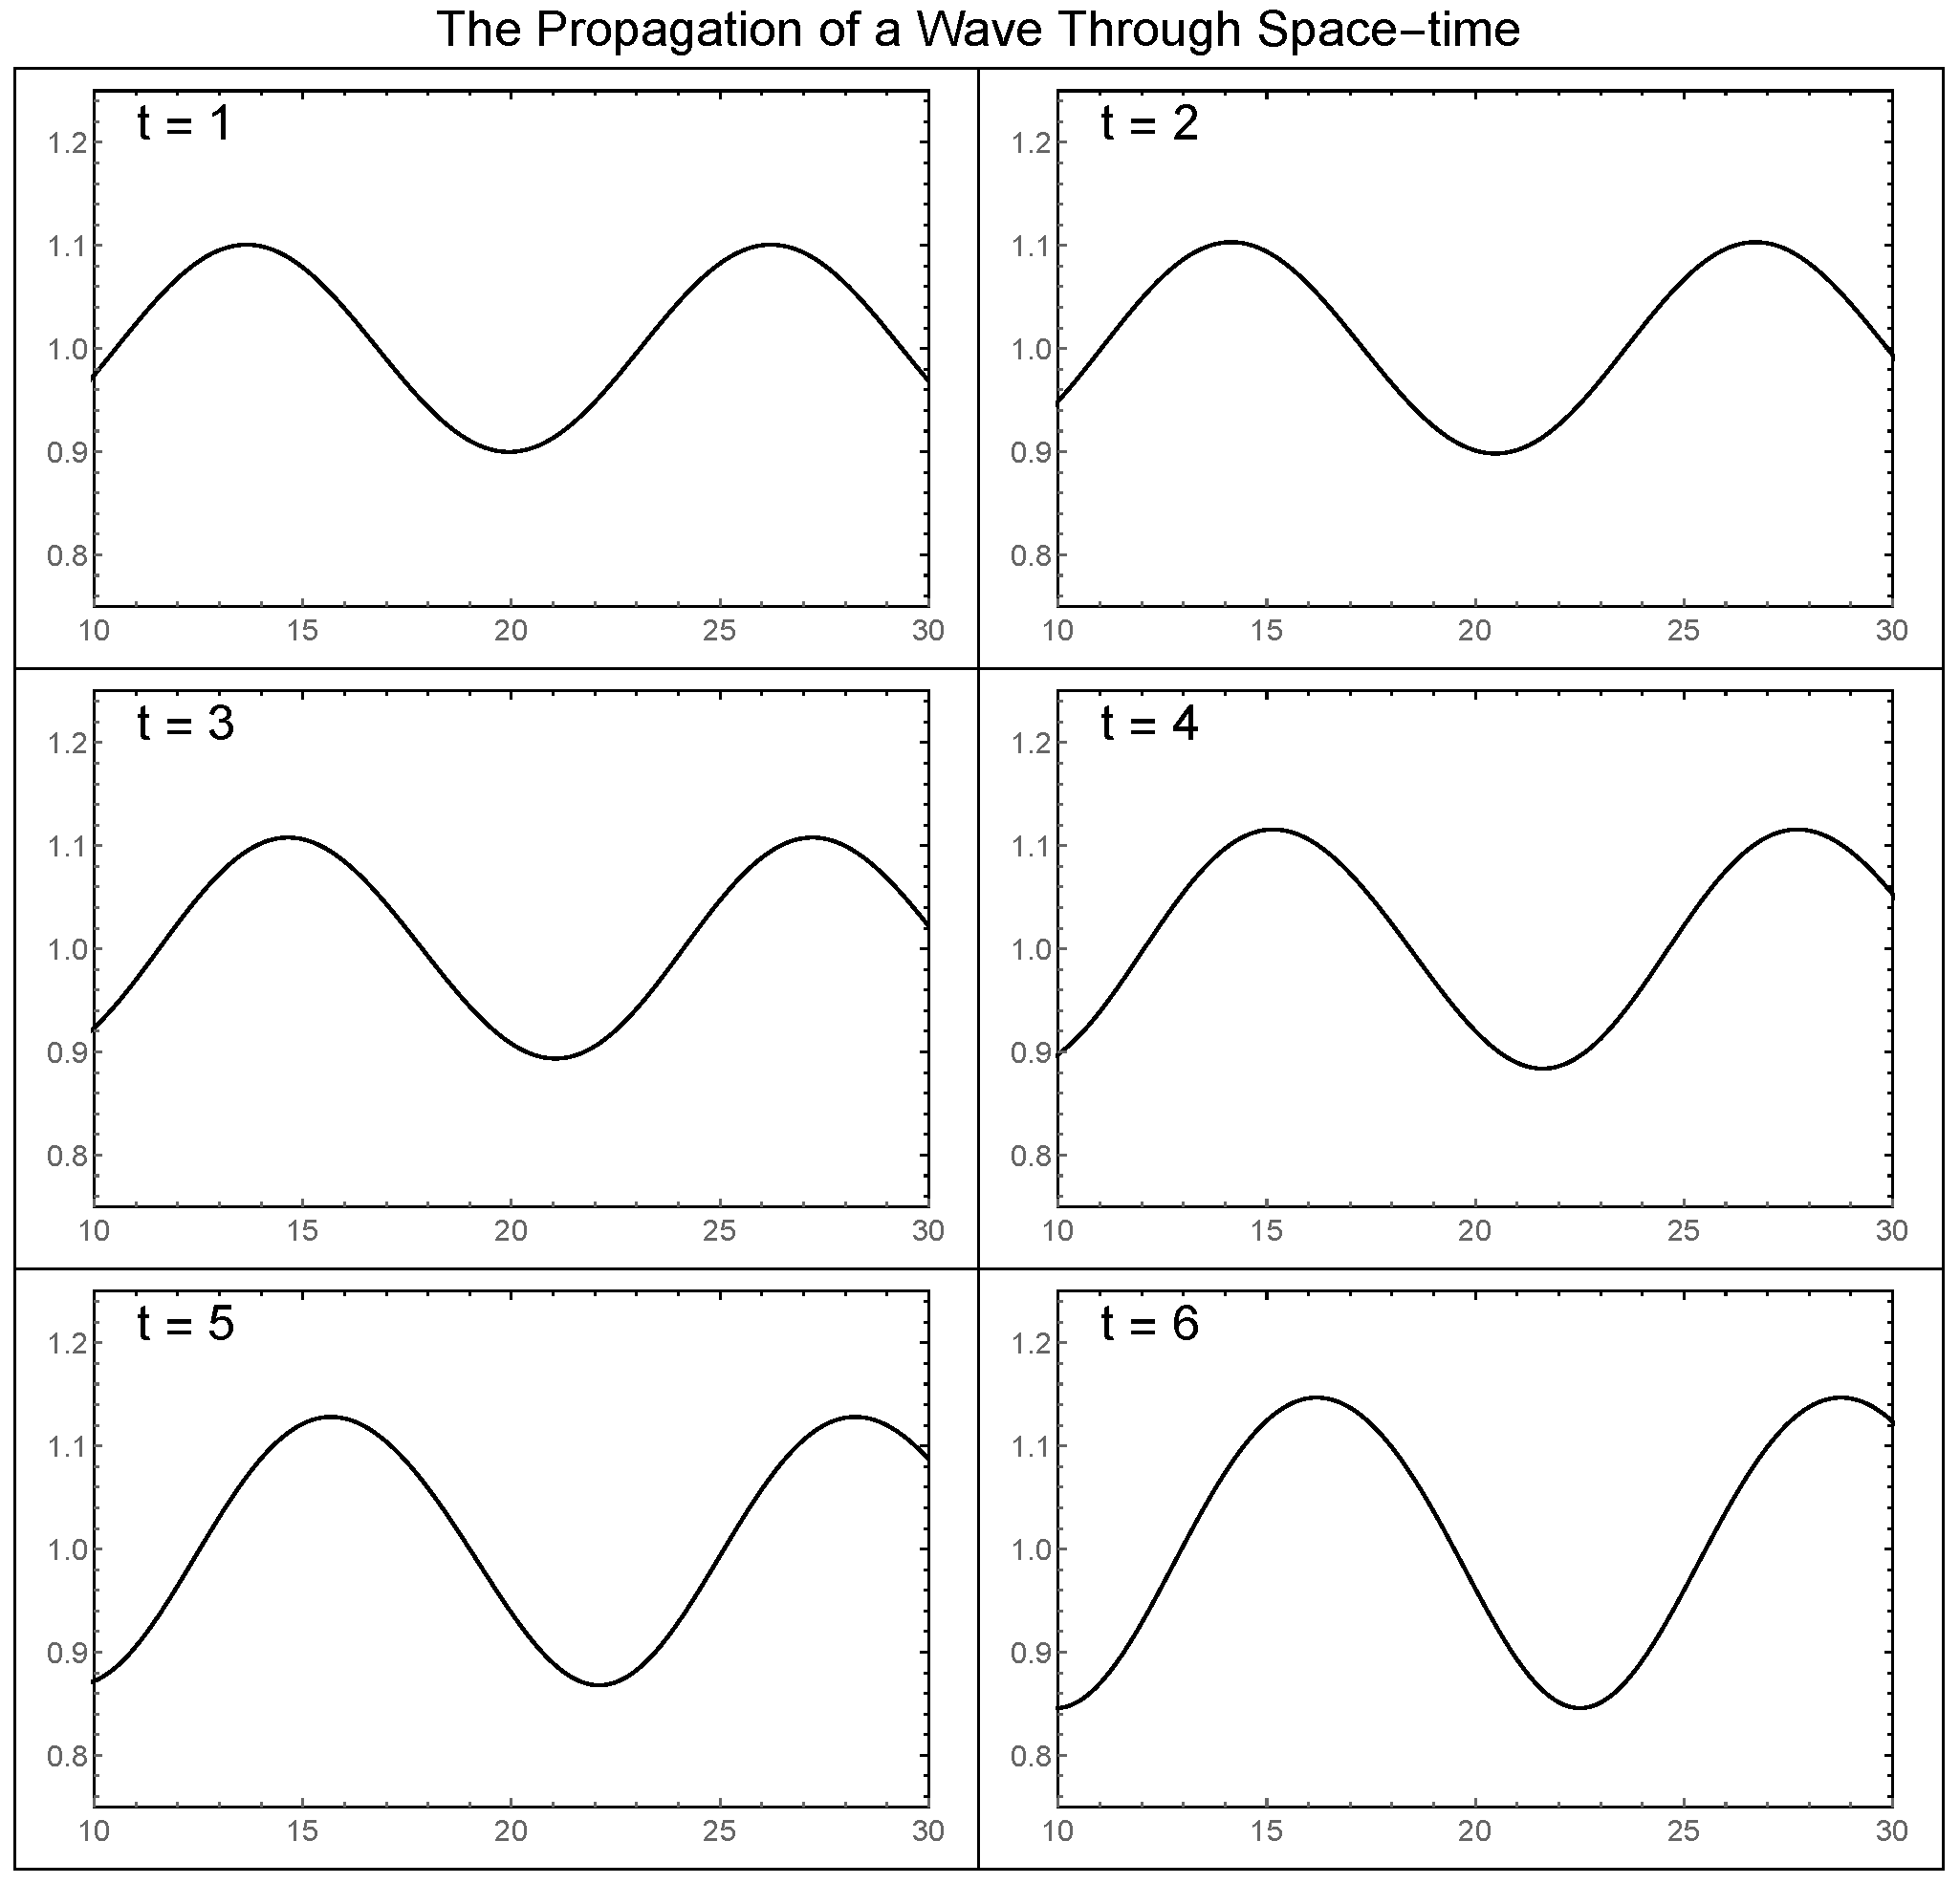
\includegraphics[width=\textwidth]{wavearray}
\caption{A wave propagating along the $x$ axis of the space time grid. Here the parameters are $k = 0.5$, $\alpha = -10.0$, and $h_p = 0.1$. It is seen that the wave moves approximately three units in the x direction.}
\end{figure}
Figure (1) shows the evolution of a sine wave defined with the initial conditions ($g^0_{22}, v^0_{22}$) as defined in equations (\ref{initcondg}, \ref{initcondv}), as it propagates in the $x$ direction of the space time grid over the period of $60$ seconds. It is seen to move the appropriate amount, about $6$ over the time interval, which is expected for the speed of the wave and time step value of $\delta t = 0.01$ for the simulation. Therefore, I have constructed a valid code that can simulate the propagation of a wave through the grid within the computational domain which is a promising result for future work on the library.

\section{Conclusion}
I have shown the basic derivations present that are used in numerical relativity, in both the $3+1$ formalism, as well as the general harmonic gauge. These derivations are then fully implemented into library, GHGFort, and used to simulate general relativistic events. GHGFort, or General Harmonic Gauge Fortran, contains modules that allow for fixed grid simulations of events in space--time. Utilizing this library a numerical simulation of a wave being propagated through space-time is successfully conducted as a proof of concept of the validity of the equations and library. The outlook of GHGFort is promising, with successful tests, these equations could be put to use to do further tests such as simulations of a static black hole using the puncture method \cite{PhysRevLett.95.121101}, and potentially merger events.

\section{Acknowledgements} 
I would like to thank my friend and mentor Dr. Justin Feng, for his immense help over the past two years in understanding the theory of general relativity, as well as guidance and immense amounts work put into writing GHGFort. I would also like to thank Mark Selover and Professor Richard Matzner, for their expertise in numerical simulations, programming, and guidance, without whose help this would also not have been possible.

Then furthermore, I would to thank my fellow students Blake Duschatko, and Avery Pawelek for their continued support and friendship throughout my undergraduate degree. 


\bibliographystyle{unsrt}
\bibliography{references}

\end{document}